% !TeX spellcheck = en_GB
\documentclass[12pt]{beamer}
\usepackage[utf8]{inputenc}
\usepackage[T1]{fontenc}
\usepackage{lmodern}
\usepackage[english]{babel}
\usepackage{amsmath}
\usepackage{amsfonts}
\usepackage{amssymb}
\usepackage{nicefrac}
\usepackage{graphicx}
\usepackage{tikz}
\usetikzlibrary{positioning}
%\usetheme{Montpellier}
%\usetheme{Berkeley}
\definecolor{std}{rgb}{0.2,0.2,0.7}
\newtheorem*{conjecture}{Conjecture}
\begin{document}
	\author{Paul Dubois}
	\title{Modular Forms Modulo 2:}
	\subtitle{Governing Fields for the Hecke Algebra}
	\logo{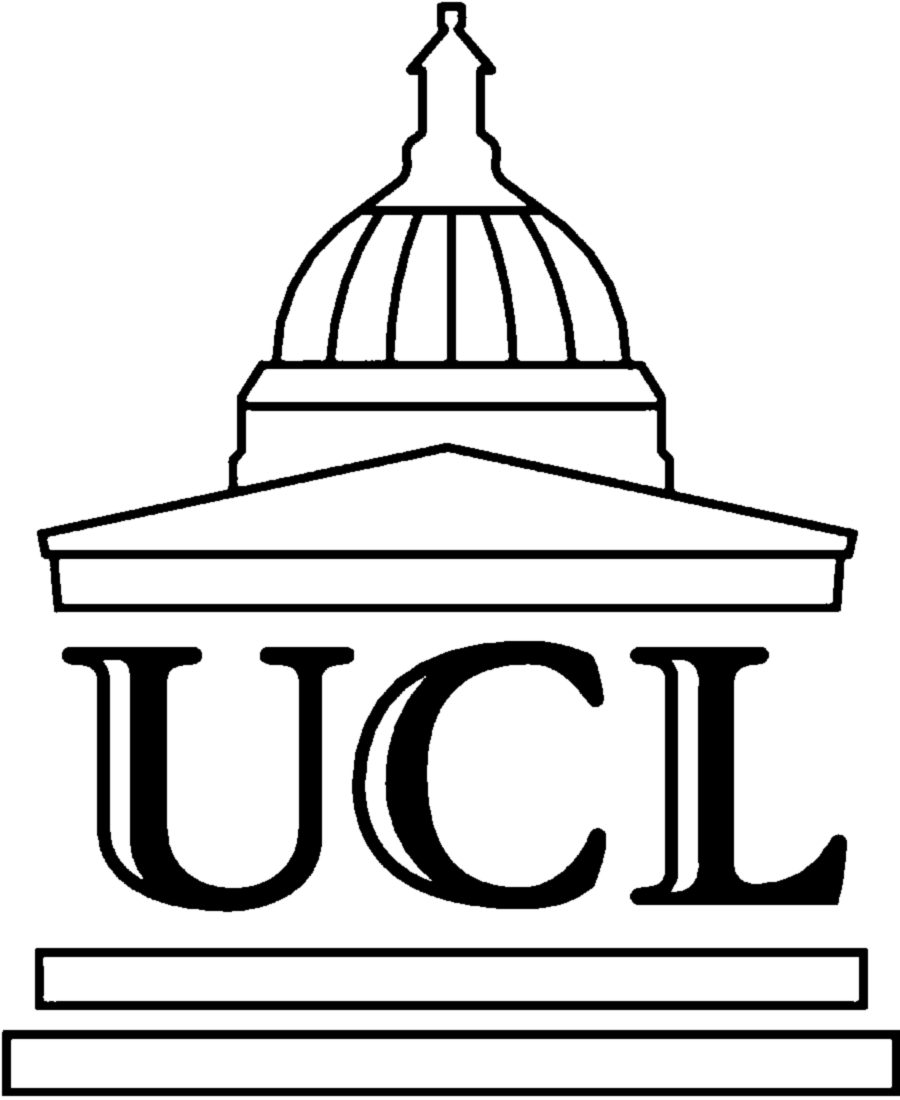
\includegraphics[scale=0.02]{ucl-logo.png}}
	\institute{University College of London}
	\date{March 25, 2020}
	\subject{Mathematics}
	%\setbeamercovered{transparent}
	%\setbeamertemplate{navigation symbols}{}
	\begin{frame}[plain]
		\maketitle
	\end{frame}
	
	\begin{frame}
		\frametitle{Modular Forms}
		\begin{center}
			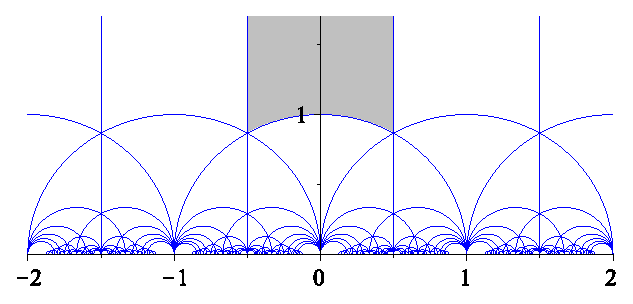
\includegraphics{ModularGroup-FundamentalDomain.eps}
		\end{center}
		
		Complex vector space of modular forms of weight $n$: $M_n$
		
		\vspace{0.5cm}
		
		For $f \in M_n$: $f(z) = \sum_{n = 0}^{\infty} c(n)q^n$ with $q^n = e^{2\pi i n z}$
	\end{frame}

	\begin{frame}
		\frametitle{Reduction Modulo 2}
		$$\left\lbrace f \in M_n \mid f = \sum_{n \in \mathbb{N}} c(n)q^n \text{ s.t. } c(n) \in \mathbb{N} \right\rbrace$$
		$$\rotatebox{90}{$=$}$$
		$$\mathbb{F}_2\left[ \Delta, E_2, E_3 \right]$$
		
		$$\overline{\Delta} \rightsquigarrow \Delta$$
		$$\overline{E_2} \rightsquigarrow 1$$
		$$\overline{E_3} \rightsquigarrow 1$$
		
		$$\overline{M_n} \rightsquigarrow \mathbb{F}_2 \left[ \Delta \right]$$
	\end{frame}

	\begin{frame}
		\frametitle{Modular Forms Modulo 2}
		$$
		\mathcal{F}
		= \left\langle \Delta^k \mid k \text{ odd} \right\rangle_{\mathbb{F}_2}
		= \left\langle \Delta, \Delta^3, \Delta^5, \dots \right\rangle_{\mathbb{F}_2}
		$$
		
		\begin{align*}
			\Delta(q)
			&= q \prod_{n=1}^{\infty} (1-q^n)^{24}\\
			&= \sum_{n=0}^{\infty} \tau(n)q^n\\
			&\equiv \sum_{m=0}^{\infty} q^{(2m+1)^2} \bmod 2\\
		\end{align*}
	\end{frame}
	
	\begin{frame}
		\frametitle{Hecke Operators}
		With
		$$
		f(q) = \sum_{n \in \mathbb{N}} c(n)q^n
		$$
		We define
		$$
		\overline{T_m}|f(q) = \sum_{n \in \mathbb{N}} \gamma(n)q^n
		$$
		Where
		$$
		\gamma(n) = \sum_{a | (n,m),\, a \geq 1} a^{2k-1} c\left( \frac{mn}{a^2} \right)
		$$
	\end{frame}

	\begin{frame}
		\frametitle{Hecke Operators Modulo 2}
		With
		$$
		f(q) = \sum_{n \in \mathbb{N}} c(n)q^n
		$$
		We define
		$$
		\overline{T_p}|f(q) = \sum_{n \in \mathbb{N}} \gamma(n)q^n
		$$
		Where
		$$
		\gamma(n) = 
		\left\lbrace
		\begin{array}{l l}
		c(np)        & \text{ if } p \nmid n \\
		c(np)+c(n/p) & \text{ if } p \mid  n
		\end{array}
		\right. 
		\quad \text{ and } p \text{ an odd prime}.
		$$
	\end{frame}

	\begin{frame}
		\frametitle{Examples}
		
		\begin{center}
			\begin{tabular}{|r|rrrrrrr|}
				\hline
				\textbf{} & \textbf{$\Delta^1$} & \textbf{$\Delta^3$} & \textbf{$\Delta^5$} & \textbf{$\Delta^7$} & \textbf{$\Delta^9$} & \textbf{$\Delta^{11}$} & \textbf{$\Delta^{13}$} \\
				\hline
				$T_3$ & 0 & $\Delta$ & 0 & $\Delta^5$ & $\Delta^3$ & $\Delta^9$ & $\Delta^7$ \\       
				$T_5$ & 0 & 0 & $\Delta$ & $\Delta^3$ & 0 & 0 & $\Delta^9$ \\
				$T_7$ & 0 & 0 & 0 & $\Delta$ & 0 & 0 & $\Delta^3$ \\
				$T_{11}$ & 0 & $\Delta$ & 0 & $\Delta^5$ & $\Delta^3$ & $\Delta + \Delta^9$ & $\Delta^7$ \\
				$T_{13}$ & 0 & 0 & $\Delta$ & $\Delta^3$ & 0 & 0 & $\Delta + \Delta^9$ \\
				$T_{17}$ & 0 & 0 & 0 & 0 & $\Delta$ & $\Delta^3$ & $\Delta^5$ \\
				$T_{19}$ & 0 & $\Delta$ & 0 & $\Delta^5$ & $\Delta^3$ & $\Delta + \Delta^9$ & $\Delta^7$ \\
				\hline
			\end{tabular}
			
			\vspace{0.5cm}
			
			\begin{tikzpicture}
[
squarednode/.style={rectangle, very thick, inner sep=0.2cm,outer sep=0},
node distance=1cm
]
\node[squarednode] (df)                    {$f = \Delta^k$};
\node[squarednode] (f)   [below=of df]     {$f = q^k + \dots$};
\node[squarednode] (Tf)  [right=3cm of f]  {$T_p|f = q^m + \dots$};
\node[squarednode] (Tdf) [right=3.415cm of df] {$T_p|f = \Delta^m + \dots$};
\draw[<->]              (df) to (f)  ;
\draw[ultra thick, ->]  (f)  to node[above] {$T_p$} (Tf) ;
\draw[<->]              (Tf) to (Tdf);
			\end{tikzpicture}
		\end{center}
	\end{frame}

	\begin{frame}
		\frametitle{The Hecke Algebra}
		\begin{align*}
			A 
			&= \mathbb{F}_2\left[ T_3, T_5, T_7, T_{11}, T_{13}, \dots \right] \\
			&= \mathbb{F}_2\left[ T_p \mid p \in \mathbb{P} \right]
		\end{align*}
		
		$$A = \mathbb{F}_2 \left[\left[ T_3, T_5 \right]\right]$$
		
		$$T_p = \sum_{i+j \geq 1} a_{ij}(p) T_3^iT_5^j$$
	\end{frame}

	\begin{frame}
		\frametitle{Examples}
		$$x = T_3 \qquad y = T_5$$
		$$\text{i.e. } x^ay^b = T_3^aT_5^b$$
		
		$T_{3} = x^{1}y^{0} = x$
		\vspace{0.2cm}
		
		$T_{5} = x^{0}y^{1} = y$
		\vspace{0.2cm}
		
		$T_{7} = x^{1}y^{1} + x^{3}y^{1} + x^{3}y^{3} + x^{5}y^{1} + x^{1}y^{7} + x^{1}y^{9} + x^{7}y^{3} + x^{7}y^{5} + x^{9}y^{3} + x^{11}y^{1} + x^{3}y^{11} + x^{5}y^{9} + x^{13}y^{1} + x^{3}y^{13} + x^{5}y^{11} + x^{9}y^{7} + x^{11}y^{5} + x^{13}y^{3} + x^{3}y^{15} + x^{7}y^{11} + x^{9}y^{9} + x^{13}y^{5} + x^{15}y^{3} + \dots $
		\vspace{0.2cm}
		
		$T_{11} = x^{1}y^{0} + x^{1}y^{2} + x^{3}y^{0} + x^{1}y^{4} + x^{3}y^{2} + x^{5}y^{0} + x^{1}y^{6} + x^{3}y^{4} + x^{7}y^{2} + x^{1}y^{10} + x^{3}y^{8} + x^{7}y^{4} + x^{9}y^{2} + x^{11}y^{2} + x^{3}y^{12} + x^{5}y^{10} + x^{7}y^{8} + x^{11}y^{4} + x^{13}y^{2} + x^{9}y^{8} + x^{17}y^{0} + \dots $
		
		\vspace{2cm}
	\end{frame}

	\begin{frame}
		\frametitle{Dirichlet Density Theorem}
		Intuition: \boxed{\href{https://pauldubois98.github.io/DirichletDensityTheoremAnimation/}{Animation}}\\
		{\tiny (see \url{https://pauldubois98.github.io/DirichletDensityTheoremAnimation/})}
		
		\vspace{1cm}
		
		\begin{theorem}[Dirichlet's Density Theorem]
			Let $n \in \mathbb{N}^*$, $a \in \mathbb{N}$ such that $\gcd(a,n) = 1$.\\
			If $S = \{ p \in \mathbb{P} \mid p \equiv a \mod n \}$, then $S$ has density $\nicefrac{1}{\varphi(n)}$.
		\end{theorem}
	\end{frame}

	\begin{frame}
		\frametitle{Chebotarev Density Theorem}
		\begin{theorem}[Chebotarev Density Theorem]
			With $L/K$ an extension of Galois group $G=\text{Gal}(L/K)$.\\
			Let $C$ be a conjugacy class in $G$.
			
			Then, the proportion of unramified primes ideals $\mathfrak{p}$ in $K$ that have Frobenius element $\text{Frob}_{L/K}(\mathfrak{p})=C$
			%\footnote{When depending on a prime in the "lower" field, the Frobenius element is a conjugacy class to be well defined.}
			is $\nicefrac{|C|}{|G|}$.
		\end{theorem}
		
		\vspace{1cm}
		
		$L = \mathbb{Q}(\zeta_n)$ and $K= \mathbb{Q}$ give Dirichlet's density theorem.
		
	\end{frame}

	\begin{frame}
		\frametitle{Frobenian Maps}
		With $K$ a number field, $P$ the set of primes in $K$.
		$f: P \to \Omega$ is Frobenian if there exists
		\begin{itemize}
			\item a set $S \subset P$
			\item a field $M$ extending $K$
			\item a class function $\phi: \text{Gal}(M/K) \to \Omega$
		\end{itemize}
		such that:
		$$f(\mathfrak{p}) = \phi( \text{Frob}_{M/K}(\mathfrak{p})) \qquad \forall \mathfrak{p} \in P \setminus S$$
	\end{frame}

	\begin{frame}
		\frametitle{The maps $a_{ij}$}
		$$T_p = \sum_{i+j \geq 1} a_{ij}(p) T_3^iT_5^j$$
		\vspace{1cm}
		$$a_{ij}: p \mapsto a_{ij}(p) \text{ is Frobenian}$$
		
		$$M_{ij} \text{ denotes a governing field for } a_{ij}$$
		$$G_{ij} \text{ denotes a governing group for } a_{ij}$$
	\end{frame}

	\begin{frame}
		\frametitle{Known identities}
		\begin{itemize}
			\item
			$a_{10}(p)=1 \iff p \equiv 3 \bmod 8$
			\item
			$a_{01}(p)=1 \iff p \equiv 5 \bmod 8$
			\item
			$a_{11}(p)=1 \iff p \equiv 7 \bmod 8$
			\item 
			$\begin{matrix}
				a_{20}(p)=1 \iff &\exists a,b \in \mathbb{Z} \text{ and } b \text{ odd},\text{ such that }\\
				&p=a^2+8b^2, p \equiv 3 \bmod 8
			\end{matrix}$
			\item
			$\begin{matrix}
				a_{02}(p)=1 \iff &\exists a,b \in \mathbb{Z} \text{ and } b \text{ odd},\text{ such that }\\
				&p=a^2+16b^2, p \equiv 3 \bmod 8
			\end{matrix}$
		\end{itemize}
	\end{frame}

	\begin{frame}
		\frametitle{Known Governing Fields}
		$$M_{01} = \mathbb{Q}\left( \zeta_8 \right)$$
		$$M_{02} = \mathbb{Q}\left( \zeta_8, \sqrt[4]{2} \right)$$
		
		$$
		M_{11}
		= \mathbb{Q}\left( \zeta_8, \sqrt{\zeta_8} \right)
		= \mathbb{Q}\left( \zeta_{16} \right)
		$$
		
		$$M_{02} = \mathbb{Q}\left(\zeta_8, \sqrt{1+i} \right)$$
		$$M_{01} = \mathbb{Q}\left(\zeta_8\right)$$
		
		\vspace{0.5cm}
		
		\begin{flushright}
			Note $\mathbb{Q}\left( \zeta_8 \right) = \mathbb{Q}\left( i, \sqrt{2} \right)$
		\end{flushright}
	\end{frame}

	\begin{frame}
		\frametitle{Potential New Governing Fields}
		$$M_{03} \stackrel{?}{=} \mathbb{Q}\left(\zeta_8, \sqrt[4]{2}, \sqrt{\alpha}\right)$$
		where:
		\begin{align*}
			\alpha =
			&- \frac{3136435454775881 \sqrt[4]{2}}{562949953421312} + \frac{4208721080340285 \sqrt{2}}{2251799813685248} +\\
			&\frac{3672578267558083 \cdot \sqrt[4]{2}^3}{562949953421312} + \frac{3582104167901087}{281474976710656}
		\end{align*}
	\end{frame}

	\begin{frame}
	\frametitle{Potential New Governing Fields}
		$$M_{05} \stackrel{?}{=}\mathbb{Q}\left(\zeta_8, \sqrt[4]{2}, \sqrt{\alpha}, \sqrt{\beta}\right)$$
		where $\alpha$ remains
%		\begin{align*}
%			\alpha =
%			&- \frac{3136435454775881 \sqrt[4]{2}}{562949953421312} + \frac{4208721080340285 \sqrt{2}}{2251799813685248} \\
%			&+ \frac{3672578267558083 \cdot \sqrt[4]{2}^3}{562949953421312} + \frac{3582104167901087}{281474976710656}
%		\end{align*}
		and
		\begin{align*}
		\beta = 
		&- \frac{8282936156772053 \alpha^{\frac{13}{2}}}{1125899906842624} 
		- \frac{1240182980093567 \alpha^{6}}{562949953421312} \\
		&- \frac{336382584949535 \alpha^{\frac{9}{2}}}{2199023255552} 
		- \frac{6445823996745319 \alpha^{4}}{140737488355328} \\
		&- \frac{4638634719581101 \alpha^{\frac{5}{2}}}{35184372088832} 
		- \frac{2954723016803317 \alpha^{2}}{70368744177664} 
		\\
		&- \frac{5142889464378747 \sqrt[4]{2}}{140737488355328} 
		- \frac{4198844765367981 \sqrt{\alpha}}{1125899906842624} \\
		&+\dots \\
%		&+ \frac{3450571136356681 \sqrt{2}}{281474976710656} 
%		+ \frac{6022015868546055 \cdot \sqrt[4]{2}^3}{140737488355328} \\
%		&+ \frac{5763554133419461}{70368744177664} 
%		+ \frac{7633450872164841 \alpha^{\frac{3}{2}}}{281474976710656} 
%		\\
%		&+ \frac{615248862392953 \alpha^{3}}{8796093022208} 
%		+ \frac{8240373942248553 \alpha^{\frac{7}{2}}}{35184372088832} \\
%		&+ \frac{8030384673908857 \alpha^{5}}{562949953421312} 
%		+ \frac{4981425151744809 \alpha^{7}}{18014398509481984} \\
%		&+ \frac{1676680829315919 \alpha^{\frac{11}{2}}}{35184372088832} 
%		+ \frac{8299866982438859 \alpha^{\frac{15}{2}}}{9007199254740992}
		\end{align*}
	\end{frame}
	\begin{frame}
		\frametitle{Governing Fields Extension Graph}
		\begin{center}
			\resizebox{\textwidth}{!}{%
			\begin{tikzpicture}[scale=0.7]
				%%%nodes
				%i+j=0
				\node at (0,0) (M00){$M_{00} = \mathbb{Q}$};
				%i+j=1
				\node at (-2,2) (M01){$M_{01}$};
				\node at (2,2) (M10){$M_{10}$};
				%i+j=2
				\node at (-4,4) (M02){$M_{02}$};
				\node at (0,4) (M11){$M_{11}$};
				\node at (4,4) (M20){$M_{20}$};
				%i+j=3
				\node at (-6,6) (M03){$M_{03}$};
				\node at (-2,6) (M12){$M_{12}$};
				\node at (2,6) (M21){$M_{21}$};
				\node at (6,6) (M30){$M_{30}$};
				%i+j=4
				\node at (-7,7) (M04){$M_{04}$};
				%\node at (-3.5,7) (M13){$M_{13}$};
				%\node at (0,7) (M22){$M_{22}$};
				%\node at (3.5,7) (M31){$M_{31}$};
				\node at (7,7) (M40){$M_{40}$};
				%i+j=5
				\node at (-9,9)(M05){$M_{05}$};
				\node at (9,9) (M50){$M_{50}$};
				%i+j=6
				\node at (-10,10) (M06){$M_{06}$};
				\node at (10,10) (M60){$M_{60}$};
				%i+j=7
				\node at (-11,11) (M07){$M_{07}$};
				\node at (11,11) (M70){$M_{70}$};
				%i+j=...
				\node at (-12,12) (M0k){$\cdots$};
				\node at (12,12) (Mk0){$\cdots$};
				%%%links
				%level 1
				\draw[-] (M00) -- (M10)node[midway, below right, rotate=45, scale=0.8] {$4$};
				\draw[-] (M00) -- (M01)node[midway, below left, rotate=-45, scale=0.8] {$4$};
				%level 2
				\draw[double] (M01) -- (M10);
				\draw[-] (M01) -- (M11)node[midway, below right, scale=0.8] {$2$};
				\draw[-] (M10) -- (M11)node[midway, below left, scale=0.8] {$2$};
				\draw[-] (M01) -- (M02)node[midway, below left, rotate=-45, scale=0.8] {$2$};
				\draw[-] (M10) -- (M20)node[midway, below right, rotate=45, scale=0.8] {$2$};
				%unknown middle
				\draw[dashed] (M11) -- (M21)node[midway, below right, scale=0.8] {?};	\draw[dashed] (M20) -- (M21)node[midway, below left, scale=0.8] {?};
				\draw[dashed] (M11) -- (M12)node[midway, below left, scale=0.8] {?};
				\draw[dashed] (M02) -- (M12)node[midway, below right, scale=0.8] {?};
				%left branch
				\draw[-] (M02) -- (M03)node[midway, below left, rotate=-45, scale=0.8] {$2$};
				\draw[double] (M03) -- (M04);
				\draw[-] (M04) -- (M05)node[midway, below left, rotate=-45, scale=0.8] {$2$};
				\draw[double] (M05) -- (M06);
				\draw[double] (M06) -- (M07);
				\draw[-] (M07) -- (M0k);
				%right branch
				\draw[-] (M20) -- (M30)node[midway, below right, rotate=45, scale=0.8] {$2$};
				\draw[double] (M30) -- (M40);
				\draw[-] (M40) -- (M50)node[midway, below right, rotate=45, scale=0.8] {$2$};
				\draw[double] (M50) -- (M60);
				\draw[double] (M60) -- (M70);
				\draw[-] (M70) -- (Mk0);
			\end{tikzpicture}
			}
		\end{center}
	\end{frame}
	
	\begin{frame}
		\frametitle{Governing Groups}
		$$
		\begin{matrix}
			G_{01} & \cong & D_{4} & \cong C_2 \times C_2 
			& \qquad &
			G_{10} & \cong & D_{4} & \cong C_2 \times C_2\\
			G_{02} & \cong & D_{8} & 
			& \qquad &
			G_{20} & \cong & D_{8} & \\
			G_{03} & \cong & D_{16} & 
			& \qquad &
			G_{30} & \cong & D_{16} & \\
			G_{04} & \cong & D_{16} & 
			& \qquad &
			G_{40} & \cong & D_{16} & \\
			G_{05} & \cong & D_{32} & 
			& \qquad &
			G_{50} & \cong & D_{32} & \\
			G_{06} & \cong & D_{32} & 
			& \qquad &
			G_{60} & \cong & D_{32} & \\
			G_{07} & \cong & D_{32} & 
			& \qquad &
			G_{70} & \cong & D_{32} & \\
		\end{matrix}
		$$
	\end{frame}

	\begin{frame}
		\frametitle{Governing Groups Extension Graph}
		\begin{center}
			\resizebox{\textwidth}{!}{%
			\begin{tikzpicture}[scale=0.7]
				%%%nodes
				%i+j=0
				\node at (0,0) (G00){$\left\lbrace Id \right\rbrace $};
				%i+j=1
				\node at (-2,2) (G01){$C_2 \times C_2$};
				\node at (2,2) (G10){$C_2 \times C_2$};
				%i+j=2
				\node at (-4,4) (G02){$D_8$};
				\node at (0,4) (G11){$D_8$};
				\node at (4,4) (G20){$D_8$};
				%i+j=3
				\node at (-6,6) (G03){$D_{16}$};
				\node at (-2,6) (G12){$G_{12}$};
				\node at (2,6) (G21){$G_{21}$};
				\node at (6,6) (G30){$D_{16}$};
				%i+j=4
				\node at (-7,7) (G04){$D_{16}$};
				\node at (7,7) (G40){$D_{16}$};
				%i+j=5
				\node at (-9,9)(G05){$D_{32}$};
				\node at (9,9) (G50){$D_{32}$};
				%i+j=6
				\node at (-10,10) (G06){$D_{32}$};
				\node at (10,10) (G60){$D_{32}$};
				%i+j=7
				\node at (-11,11) (G07){$D_{32}$};
				\node at (11,11) (G70){$D_{32}$};
				%i+j=...
				\node at (-12,12) (G0k){$\cdots$};
				\node at (12,12) (Gk0){$\cdots$};
				%%%links
				%level 1
				\draw[-] (G00) -- (G10)node[midway, below right, rotate=45, scale=0.8] {$4$};
				\draw[-] (G00) -- (G01)node[midway, below left, rotate=-45, scale=0.8] {$4$};
				%level 2
				\draw[double] (G01) -- (G10);
				\draw[-] (G01) -- (G11)node[midway, below right, scale=0.8] {$2$};
				\draw[-] (G10) -- (G11)node[midway, below left, scale=0.8] {$2$};
				\draw[-] (G01) -- (G02)node[midway, below left, rotate=-45, scale=0.8] {$2$};
				\draw[-] (G10) -- (G20)node[midway, below right, rotate=45, scale=0.8] {$2$};
				%unknown middle
				\draw[dashed] (G11) -- (G21)node[midway, below right, scale=0.8] {?};	\draw[dashed] (G20) -- (G21)node[midway, below left, scale=0.8] {?};
				\draw[dashed] (G11) -- (G12)node[midway, below left, scale=0.8] {?};
				\draw[dashed] (G02) -- (G12)node[midway, below right, scale=0.8] {?};
				%left branch
				\draw[-] (G02) -- (G03)node[midway, below left, rotate=-45, scale=0.8] {$2$};
				\draw[double] (G03) -- (G04);
				\draw[-] (G04) -- (G05)node[midway, below left, rotate=-45, scale=0.8] {$2$};
				\draw[double] (G05) -- (G06);
				\draw[double] (G06) -- (G07);
				\draw[-] (G07) -- (G0k);
				%right branch
				\draw[-] (G20) -- (G30)node[midway, below right, rotate=45, scale=0.8] {$2$};
				\draw[double] (G30) -- (G40);
				\draw[-] (G40) -- (G50)node[midway, below right, rotate=45, scale=0.8] {$2$};
				\draw[double] (G50) -- (G60);
				\draw[double] (G60) -- (G70);
				\draw[-] (G70) -- (Gk0);
			\end{tikzpicture}
			}
		\end{center}
	\end{frame}

	\begin{frame}
		\frametitle{Diagonal Governing Groups}
		\begin{conjecture}[Diagonal Governing Groups Conjecture]
			For all $k \in \mathbb{N}^*$, there exists a field $M_{0k}$ such that $M_{0k}$ is a governing field for $a_{0k}$, and $G_{0k} = \text{Gal}(M_{0k}/\mathbb{Q})$ is dihedral.\\
			For all $k \in \mathbb{N}^*$, there exists a field $M_{k0}$ such that $M_{k0}$ is a governing field for $a_{k0}$, and $G_{k0}$ is dihedral.\\
			\ \\
			Moreover $M_{k0} \neq M_{0k}$ in general, but $G_{k0} \cong G_{0k}$.
		\end{conjecture}
	\end{frame}

	\begin{frame}[plain]
		\begin{center}
			{\Large \color{std} Thank you}
		\end{center}
	\end{frame}



\end{document}